\chapter{Requirements and Challenges}
\label{ch:rqrmsandclngs}

After analysing the different approaches taken by previous work, we define a number of requirements and challenges our solution has to meet and overcome. Most of these generate complexity in the system, and make for potential issues for long term support. For this reason, we first discuss the requirements that drive our choices when facing the challenges this project presents, and finally we validate the decisions we take to overcome these issues.

\section{Requirements}
\label{sec:rqrmsandclngs-requirements}

In order to develop the environment we envision, we first define the requirements our software meets. We present them under four umbrella terms representing how they impact our choices and process. Under these umbrellas, we explain how in particular these impact our solution, and define the necessary terminology we use.

\subsection{Usability}

As first and foremost, Usability is the key requirement of our environment. As one of our objectives is to lower the technical barrier to developing VR applications, the software we present needs to be crafted with particular care to its usability. The issue with this, is the difficulty we have defining what usability is in the first place. A number of definitions have been proposed in the past, though scope of the term is yet to be determined \cite{8279761}. Thus, in order to avoid ambiguity, we refer to the term as defined in the ISO/IEC 25010:2011:

\begin{quote}
    \textbf{Usability} Degree to which a product or system can be used by specified users to achieve specified goals with effectiveness, efficiency and satisfaction in a specified context of use \cite{25010:2011}.
\end{quote}

As we develop our environment, we consider two levels of usability of our software. The first level, or high level, refers to the usability as seen from the end-user who has no or low technical knowledge and needs our environment to develop his application, thus refering to the UI of the environment. The second level, or low leve, refers to the usability as seen from a skilled user who has technical knowledge and aims at modifying or expanding the environment, or use it with more freedom, and thus develops also with code within our environment.

As such, to cater to the high level usability, the software should be usable out of the box. In particular, the UI should be intuitive and easy to use. For this reason, the use of Heds-Up Displays (HUD) within the VR environment should be limited, to avoid cluttering the user's viewport, and the tools should be part of the environment, interactable and movable, in order to make all the environment's objects tools that the user can use in similar way. This also limits the number of gestures and inputs the user has to memorize, as well as having adaptable and customizable configurations of what information the UI should show and where this is avaialable, making the experience tailored to the user.

However, as our main focus is the engine, we also define the low level requirements, as this remains the main access-point to VTK used in the environment. In particular, the API of our software should be as expressive as possible, meaning the user can write any software the usage of just VTK would allow them. Furthermore, the information inserted in the API should be as explicit as possible, limiting black box operations the user is not informed of, and limiting the need for further documentation. For example, the types in which the parameters are expressed in generic calls should be explicitly specified in the function calls, with constants avaiable to the user that represent these types, without them having to query the documentation in order to know how this representation works.

\subsection{Generality}

To lower the coupling between our software and \acrshort{vtk}, we want it to be version-agnostic. This coupling is already weakened by the fact the library is developed to be backwards-compatible and the only major change to the API that broke this, happened between versions 4 and 6 of the library\footnote{\url{https://vtk.org/Wiki/VTK/VTK\_6\_Migration/Overview}.}. In order to make the software version-agnostic, the access to the library should be general, i.e. our solution should limit direct calls to VTK's API, prefering adaptable solutions, e.g. introspection, adapter generation, etc.

As usability is also one of the requirements of our software, the benefits of a general access approach are not limited to its maintainability, and generality as a whole also impacts the usability of the environment, as the other way around is true. Refering to the high level usability, we presented an example refering to the UI of the environment. Such UI was also described as general, as it would be composed of environment objects that could be rearrenged by the user to customize its own workstation. We mirror this approach of customizability and generality to all the aspects of our solution.

This is al the more critical when looking at the way we interface with VTK. Hardcoding its features would possibly make for the best performances, but would make the system a huge collection of functions, as it would be necessary to wrap the calls for every class and method accessible to the user. Making the access to VTK general would both boost its version-agnosticism as well as its maintainability.

Expanding on the UI, the system should be able to show a UI for any type of operation the user can execute with VTK. The user should not be responsible for implementing UI components for VTK features that are not foreseen in our code, and as such the way the UI is handled and generated should also be general, it should be able to generate necessary components on-the-fly. This is also part of the full access we just presented in the previous paragraph. In terms of usability, full access makes the environemnt usable at low level, whereas UI generation at high level.

\subsection{Maintainability}

In order to have a maintainable system, we have to take into consideration a number of metrics and apply conventions that make our solution more robust and enable long-term support. In particular, we focus on N characteristics, some of which we want to minimize, some maximize, that we see fit to achieve these two objectives. We aim at minimizing \acrfull{slocs}, that measure the size of the code base in lines of source code, and coupling with external software, and at maximizing separation of concerns and readability.

One of the main metrics we use to measure the maintainability, is its \acrlong{slocs}. These have a strong connection to the maintainability of the codebase and as such we aim at keeping its value low \cite{4335232}. We aim at achieving this by limiting code clones and re-using code wherever possible. Based on the Software Improvement Group's Maintainability Model, a codebase below 322 thousand SLOCs\footnote{Based on V13 (May 26, 2021) Evaluation criteria \url{https://www.softwareimprovementgroup.com/methodologies/iso-iec-25010-2011-standard/}.}.

Another metric we aim at keeping low is coupling. In particular, we aim to keep the coupling level loose by having data coupling with external libraries and reducing the number of libraries necessary \cite{8016712}. Furthermore, we aim at lowering the impact of these couplings by using the Facade Pattern and keeping the coupling at the edges of the software \cite{alma990009471180205131}. The internal coupling of the system is necessarily common-environment coupling as data has to be accessed directly from different modules, i.e. for efficient rendering and updating purposes.

In order to keep the software maintainable, it should be easy for a developer to clearly understand the code. For this reason, we use some coding conventions in order to make the code more comprehensible. First and foremost, each function should come with a comment clearly specifying the responsibility of the function and what it should be used for. Moreover, the size of each function should be as short, and its responsibilities as concise as possible.

Finally, function and methods should cater to as little and consice responsibilitiies as possible, being focused on very few things. This may clash with our aim at keeping the SLOCs count low, but it balances of the complexity introduced in small yet packed functions that enact a lot of responsibilities. This may also create interface duplication, as multiple layers expose similar functionality but wrapped in further decorating information. For this reason we introduce a convention on how the interfaces should be specified.

\subsection{Performance}

Our final requirement for our solution is that it is performant. This is particularly important as for a decent user experience with VR applications, these should aim at a stable FPS that mirrors the HMD's refresh rate. In general, the target should be 90 FPS as most HMDs have a 90 Hz refresh rate\footnote{Some HMDs may come in varying refresh rates, a list of devices with relative specifications is available \url{https://en.wikipedia.org/wiki/Comparison_of_virtual_reality_headsets}.} \cite{unity_vr_2020}. Another aspect of performance is memory usage. As VTK objects may become memory-heavy, we should limit how much overhead we introduce on the memory. However, this is a soft requirement, as it may not be possible to achieve decent time performances without keeping a lot of information readily available, and time performance is more critical for user experience.

However, hardcoding \acrshort{vtk}s features would make for the best performances, but would make the system plugin a huge collection of functions, as it would be necessary to wrap the calls for every class and method accessible to the user, which is hardly what we aim at. As such, we must accept a compromise between the two, however the objective of a stable 90 FPS is critical for this project.

\section{Challenges}
\label{sec:rqrmsandclngs-challenges}

Given the requirements of the system we aim to create, there a number of challenges we must face before implementing the software. These are mostly related to its design and technology choices, and as such we will discuss them separately from the actual implementation. These challenges mainly relate to the issue of connecting VTK and Unity and to the ability to guarantee full access to VTK from Unity while upholding version-agnosticism.

\subsection{Unity Integration}

The foremost factor of complexity and maintainability issues is the integration of the system with the Unity Engine. Integrating two rendering components is challenging in two main ways. First to tackle is the issue of sharing resources and the rendering context, as taken separately Unity and \acrshort{vtk} have both their own objects, memory spaces and rendering contexts.

To simplify the issue, we can make our solution a part of the Unity environment we are developing by creating a Unity native plugin. These are libraries written in C, C++ or Objective-C that are not constrained by the Unity environment like C\# Managed plugins \cite{technologies_21AD}. By making our solution a Unity native plugin, we now have to solve the problem of sharing data between the rendering contexts of Unity and \acrshort{vtk}.

As we are taking a similar approach to Wheeler et al.'s, we also follow their solution to solve this issue. In VtkToUnity the sharing of resources between the two rendering contexts is achieved using OpenGL Core ES technology, as it allows for sharing some objects between OpenGL Core conforming contexts \cite{wheeler_virtual_2018}. As the specification of these contexts is forward compatible, we also do not need to worry about compatibility between versions \cite{khronos_opengl_2021}.

We use as base for our software Wheeler's VtkToUnity plugin, as such we use the same system they developed for sharing data between rendering context and for integrating the event loops of Unity and \acrshort{vtk}. This second issue was also tackled by Wheeler et al. by nesting the \acrshort{vtk} event loop iteration in Unity's using the engine's event queue event handlers and graphics callbacks \cite{wheeler_virtual_2018}. The obtained architecture for the plugin is shown in Figure~\ref{fig:wheeler-architecture}. Most of the functionality handling these loops is implemented in the C\# scripts of Unity, which call the correct native function from the plugin in order to trigger the corresponding event in \acrshort{vtk}. A zoom in of the architectural specification can be seen in Figure~\ref{fig:wheeler-architecture-zoomin} where the particular calls from the scripts is highlighted and what is called in \acrshort{vtk} as a consequence for a particular Unity scene developed by Wheeler et al. \cite{wheeler_virtual_2018}.

\begin{figure}[t]
    \centering
    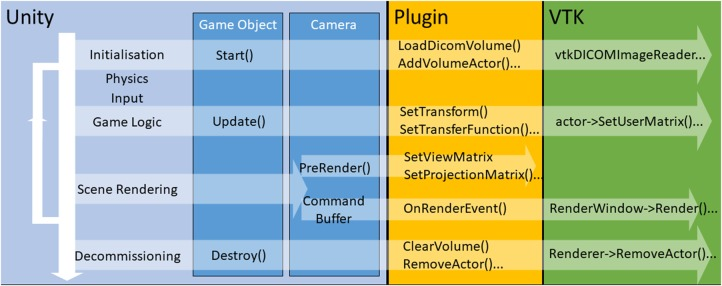
\includegraphics[width=\textwidth]{pictures/wheeler_architecture_zoomin.jpg}
    \caption{Wheeler et al.'s script handling of the VTK event loop.}
    \label{fig:wheeler-architecture-zoomin}
\end{figure}

\subsection{VTK Completeness}

As already introduced, we aim at fully exposing VTK's functionality to the Unity environment. More formally, we define VTK completeness as the characteristic of an environment that is able to access the full extent of the VTK library, whether it was or not built with its optional modules, and can produce the same visualizations as a native C++ application using VTK would be able to. 

In order to achieve such a property, we either generate adapters for all possible software components of VTK that are to be exposed, or we design a system that is able to generically access this information at runtime. As the first makes the system more coupled to the version of VTK with which it is built, and as such adapters are to be generated every time the system is built, it hardly fits our requirements. Thus, we choose to use introspection as our access system to the features of VTK.

As our system uses a C++ plugin to integrate VTK and Unity, and this language does not present an introspective interface, we need to give it access to this feature. The main issue of trying to introduce introspection capabilities to C++ is its memory handling. In particular, non-intrusive solutions that do not require modifications to the compiler generate memory overheads \cite{bayser2012rtti} and/or do not present complete introspection systems, as constructs such as \verb|union| cannot be easily handled \cite{tyng1998nonintrusive}.

Using solutions that would modify the C++ compiler are also not of our interest as they introduce a very tight coupling with the modificiations in place, and potential for unexpected breaking points down the development process that would not be easily traceable back to these modifications. For these reasons we see these solutions as non-starters for our project. Thus, we need to introduce introspection through a further module.

Our approach aims to integrate Dreuning's Python introspection scripts \cite{dreuning_visual_2016} within the C++ native plugin, as this would still allow for a performing system written in C++ to access Python's capabilities when it is necessary to expose parts of \acrshort{vtk} the system. The solution presented by Dreuning is able to achieve decent performances in Python, and has the characteristics we need.

\subsection{Integrating C++ and Python}

Introducing these Python scripts within the C++ plugin can be achieved through two different approaches: keeping the Python component separate and make it communicate with the C++ native plugin or embedding the Python interpreter within the C++ code itself.

The option of syncrhonizing different modules would be best for maintainability purposes, as it would maximize separation of concerns, as well as isolating modules and reducing coupling, as they would need to synchronize data at worst, whereas the embedding of the Python interpreter would make the coupling tighter. This being said, the redundancy of data created introduces a memory overhead that is not negligible. This overhead is necessary as the VTK objects would need to be accessible from both components, and as separate modules they would need to synchronize them. 

With the embedding, the issue would be to share the memory area of the VTK objects of the C++ plugin with the Python interpreter. This is made easy by VTK though, as the wrapped Python objects keep a reference to the C++ objets they wrap. This allows us to embed the interpreter within the program's memory area and avoids us to have to manually manage the sharing of objects between the two parts. As such, we opt to embed the Python interpreter as it makes for the best performances and does not impair maintainability to a signifcant degree.

\subsection{Python/C API}

As the developers of Python already foresaw a use for Python tightly coupled with other languages, as well as the possibility for users to extend the language, the interpreter can be embedded using natively supported calls that are part of what is called the Python/C API \cite{python_c_api}. This API gives access to the ability to instantiate a Python interpreter within a C/C++ software that shares with the interpreter its memory, in order to allow both to access data in a fast and controlled manner.

However, this API is verbose, especially while working with objects, which made us consider the usage of a third party library called Boost::Python, which extends the Python/C API, further simplifying the embedding of the interpreter. The most useful feature which would immensily aid the maintainability and readability of our code is its automatic handling of the Python reference count of objects.

In order for Python's garbage collector to properly dispose of an object, the language decorates each instance with a reference count, which is a counter that keeps track of how many variables are referencing the object. Once this counter reaches zero, the garbage collector disposes of it and frees its memory. The Python/C API leaves the handling of these counters to the user through the usage of \verb|Py_DECREF| and \verb|Py_INCREF| macros.

While this freedom allows for more sophisticated uses of the interface, it also makes the code more complex to read, making the codebase larger in terms of SLOCs and more complex as it requires controlling references and being careful not to create memory leaks. This is made more complicated as some functions of the API increase the reference count while others \textit{steal} its reference from the caller, making the system prone to memory leaks. This is somewhat helped by the introduction of the \verb|Py_XDECREF| macro which decreases if not null or already zero.

On the other hand, while Boost::Python aids in making the code more readable and maintainble, it also introduces a further coupling with a third party library, which is comprised of a multitude of functionality that is not required for our software, introducing breaking points. Furthermore, the structures wrapped around \verb|PyObject|, the controls and the exception handling system introduced by the library results in overhead on both memory and speed of the execution, which is not ideal in our performance-critical environment. 

For even further support, \acrshort{vtk} ships with a module to facilitate Python/C++ integrations exposing functions that easily wrap C++ and unwrap Python \acrshort{vtk} objects, as each wrapped Python object keeps a reference to the C++ object, and from the pointer to the object the wrapper can be generated.

%TODO:Should I leave this here or move it to Future work?
As a proof of concept, to showcase the capabilities of our system, we do not use Boost::Python, so to limit external coupling and overheads and because VTK alreadyh offers an integration of the API that makes the usage of the Python/C API easier. We recognise though that the advantages of the library are not trivial and it should be explored as a potential option for future updates to the project.

\section{Validation}
\label{sec:rqrmsandclngs-validation}

Before discussing design and implementation of our plugin, we validate our choices to tackle the challenges we face in this project. Because we base our plugin on VtkToUnity, the integration with Unity through the usage of a native plugin is already validated by their results, achieving the recommended performance of 90 FPS. On the other hand, the validation of the Python embedding choice is not available, and as such we develop a small test confirming our choice.

\subsection{Python Embedding tests}

On the other hand, the embedding of the Python interpreter is a common choice and is discussed in the official guidelines of Python itself\footnote{\url{https://docs.python.org/3/extending/embedding.html}} and can achieve decent performances. In order to determine the overhead introduced by the embedding, we compare the execution times of an embedded application with the same application in pure Python and repeat this for direct access to \acrshort{vtk} and using the Dreuning's introspection scripts.s

The application we run is a stream tracer of a density dataset for \acrshort{vtk} applications. The final visualization is composed of the outline and the streamlines. The pipeline can be seen in Figure~\ref{fig:streamtracer_pipeline}. This pipeline has been implemented in Python 3.7 directly using the \acrshort{vtk} library and accessing it through a modified and expanded version of Dreuning's scripts, the embedded verion of the Python interpreter in C++ executing Python calls directly to \acrshort{vtk}, and finally again through C++ by calling the functionality exposed by the modified Dreuning's scripts. The code for each of these tests is presented in Appendix~\ref{apx:streamtracer-performance-tests} and the results are shown in Table~\ref{tab:streamtracer-performance-tests-results}.

\begin{figure}[t]
    \centering
    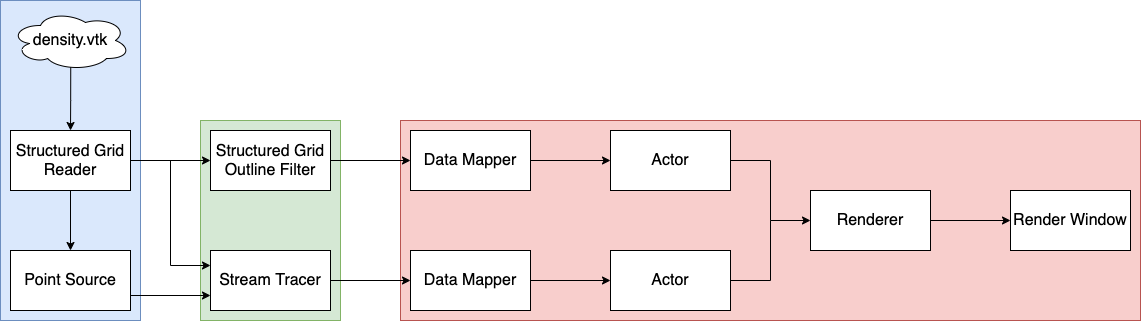
\includegraphics[width=\textwidth]{pictures/streamtracer_pipeline.png}
    \caption{VTK pipeline of a Stream Tracer on a density dataset.}
    \label{fig:streamtracer_pipeline}
\end{figure}


\begin{table}[t]
  \centering
  \caption{Performance tests' results using Python and C++ with and without introspection, implementing the pipeline from Figure~\ref{fig:streamtracer_pipeline}. Each benchmark has been run 1000 times.\\
  {\footnotesize*: time required to load the necessary structures for embedding Python and using the Introspector.\\
  **: cumulative times of the specified operation type.}}
  \label{tab:streamtracer-performance-tests-results}
  \begin{subtable}{\textwidth}
    \centering
    \caption{Python 3.7.8 implementation accessing directly VTK resources and methods.}
    \label{tab:python-native-tests}
    \resizebox{.84\textwidth}{!}{
    \begin{tabular}{llllll}
      \multicolumn{1}{c}{} &
      \multicolumn{1}{c}{\textbf{mean}} &
      \multicolumn{1}{c}{\textbf{std}} &
      \multicolumn{1}{c}{\textbf{min}} &
      \multicolumn{1}{c}{\textbf{50\%}} &
      \multicolumn{1}{c}{\textbf{max}} \\ \hhline{======}
    \textbf{Loading*}             & 0          & 0        & 0          & 0          & 0          \\
    \textbf{Instantiation**}      & 0.346051   & 0.014965 & 0.316300   & 0.343050   & 0.435700   \\
    \textbf{Update}               & 525.841453 & 7.759079 & 510.060500 & 525.217500 & 616.136600 \\
    \textbf{Setting**}            & 0.032811   & 0.001585 & 0.030600   & 0.032500   & 0.058100   \\
    \textbf{Getting**}            & 0.214747   & 0.012234 & 0.201500   & 0.209500   & 0.304900   \\
    \textbf{Connecting**}         & 0.026682   & 0.002228 & 0.022300   & 0.026300   & 0.044900   \\
    \textbf{Finalizing*}          & 0          & 0        & 0          & 0          & 0          \\ \hline
    \textbf{Total execution time} & 526.718930 & 7.764707 & 510.964400 & 526.091400 & 617.007400 \\ \hline
    \textbf{VTK execution time}   & 526.718930 & 7.764707 & 510.964400 & 526.091400 & 617.007400
    \end{tabular}}
  \end{subtable}
  \vspace*{.5truecm}
  \newline
  \begin{subtable}{\textwidth}
    \centering
    \caption{Python 3.7.8 implementation accessing VTK through introspection.}
    \label{tab:python-introspection-tests}
    \resizebox{.84\textwidth}{!}{
    \begin{tabular}{llllll}
    \multicolumn{1}{c}{} &
      \multicolumn{1}{c}{\textbf{mean}} &
      \multicolumn{1}{c}{\textbf{std}} &
      \multicolumn{1}{c}{\textbf{min}} &
      \multicolumn{1}{c}{\textbf{50\%}} &
      \multicolumn{1}{c}{\textbf{max}} \\ \hhline{======}
    \textbf{Loading*}             & 1890.429543 & 19.276412 & 1847.309400 & 1887.602000 & 2059.148200 \\
    \textbf{Instantiation**}      & 0.732206    & 0.030549  & 0.684000    & 0.726600    & 1.064900    \\
    \textbf{Update}               & 527.823380  & 9.644450  & 512.147300  & 526.707950  & 652.077100  \\
    \textbf{Setting**}            & 0.068662    & 0.003141  & 0.064600    & 0.068100    & 0.110400    \\
    \textbf{Getting**}            & 0.220781    & 0.012619  & 0.208500    & 0.215800    & 0.341100    \\
    \textbf{Connecting**}         & 0.026044    & 0.003457  & 0.022300    & 0.024800    & 0.053600    \\
    \textbf{Finalizing*}          & 0           & 0         & 0           & 0           & 0           \\ \hline
    \textbf{Total execution time} & 2421.561489 & 23.739328 & 2362.667700 & 2417.877550 & 2611.760000 \\ \hline
    \textbf{VTK execution time}   & 531.131946  & 9.659824  & 515.358300  & 529.996600  & 655.820200 
    \end{tabular}}
  \end{subtable}
  \vspace*{.5truecm}
  \newline
  \begin{subtable}{\textwidth}
    \centering
    \caption{C++11 implementation embedding Python accessing directly VTK resources and methods.}
    \label{tab:cpp-native-tests}
    \resizebox{.84\textwidth}{!}{
    \begin{tabular}{llllll}
    \multicolumn{1}{c}{} &
      \multicolumn{1}{c}{\textbf{mean}} &
      \multicolumn{1}{c}{\textbf{std}} &
      \multicolumn{1}{c}{\textbf{min}} &
      \multicolumn{1}{c}{\textbf{50\%}} &
      \multicolumn{1}{c}{\textbf{max}} \\ \hhline{======}
    \textbf{Loading*}             & 336.828093 & 8.202800 & 322.595000 & 334.397500 & 399.382000 \\
    \textbf{Instantiation**}      & 0.298408   & 0.015259 & 0.264000   & 0.298000   & 0.412600   \\
    \textbf{Update}               & 0.003026   & 0.000261 & 0.002600   & 0.003000   & 0.007400   \\
    \textbf{Setting**}            & 0.033670   & 0.004690 & 0.030800   & 0.033400   & 0.135800   \\
    \textbf{Getting**}            & 0.003260   & 0.000307 & 0.002500   & 0.003200   & 0.005100   \\
    \textbf{Connecting**}         & 0.005054   & 0.000793 & 0.004200   & 0.005000   & 0.026200   \\
    \textbf{Finalizing*}          & 17.801718  & 0.535997 & 16.879800  & 17.667700  & 21.718900  \\ \hline
    \textbf{Total execution time} & 355.044973 & 8.151684 & 341.223000 & 352.565000 & 421.322000 \\ \hline
    \textbf{VTK execution time}   & 0.415162   & 0.020545 & 0.370700   & 0.415450   & 0.548600  
    \end{tabular}}
  \end{subtable}
  \vspace*{.5truecm}
  \newline
  \begin{subtable}{\textwidth}
    \centering
    \caption{C++11 implementation embedding Python accessin VTK through introspection.}
    \label{tab:cpp-introspection-tests}
    \resizebox{.84\textwidth}{!}{
    \begin{tabular}{llllll}
    \multicolumn{1}{c}{} &
      \multicolumn{1}{c}{\textbf{mean}} &
      \multicolumn{1}{c}{\textbf{std}} &
      \multicolumn{1}{c}{\textbf{min}} &
      \multicolumn{1}{c}{\textbf{50\%}} &
      \multicolumn{1}{c}{\textbf{max}} \\ \hhline{======}
    \textbf{Loading*}             & 2247.011260 & 28.316549 & 2197.630000 & 2241.280000 & 2522.560000 \\
    \textbf{Instantiation**}      & 0.666370    & 0.033469  & 0.614600    & 0.655350    & 0.966600    \\
    \textbf{Update}               & 267.402500  & 4.770508  & 258.869000  & 266.831000  & 316.591000  \\
    \textbf{Setting**}            & 0.077507    & 0.004178  & 0.070100    & 0.076400    & 0.119000    \\
    \textbf{Getting**}            & 0.279808    & 0.017314  & 0.255800    & 0.274200    & 0.447800    \\
    \textbf{Connecting**}         & 0.047544    & 0.006922  & 0.036400    & 0.046900    & 0.187700    \\
    \textbf{Finalizing*}          & 23.925579   & 0.989636  & 23.330900   & 23.770100   & 45.308700   \\ \hline
    \textbf{Total execution time} & 2539.422550 & 30.844464 & 2488.160000 & 2533.210000 & 2825.620000 \\ \hline
    \textbf{VTK execution time}   & 268.485711  & 4.784796  & 259.920400  & 267.901450  & 317.774000 
    \end{tabular}}
  \end{subtable}
\end{table}


  % \begin{table}[t]
  %   \caption{Performance test results on Python and C++ using VTK with and without introspection.\\
  %   *: time required within the execution to load the necessary structures for embedding Python and using the Introspector.\\
  %   **: average times calculated on the different methods used within the code.}
  %   \centering
  %     \begin{tabular}{lllll}
  %     \hline
  %     \multicolumn{1}{c}{\multirow{2}{*}{\textbf{Operations}}} &
  %       \multicolumn{2}{c}{\textbf{Python}} &
  %       \multicolumn{2}{c}{\textbf{C++}} \\ 
  %     \multicolumn{1}{c}{} &
  %       \multicolumn{1}{c}{\textbf{Native}} &
  %       \multicolumn{1}{c}{\textbf{Introspection}} &
  %       \multicolumn{1}{c}{\textbf{Native}} &
  %       \multicolumn{1}{c}{\textbf{Introspection}} \\ \hhline{=====}
  %     Loading*                       & \multicolumn{1}{l}{0}         & 1.8973614 & 0.7491320 & 2.7688682 \\
  %     Object instantiation**         & \multicolumn{1}{l}{0.0046789} & 0.0001833 & 0.0000791 & 0.0001782 \\
  %     Reader update                  & \multicolumn{1}{l}{0.5265901} & 0.5276741 & 0.0000029 & 0.2713980 \\
  %     Attribute setting**            & \multicolumn{1}{l}{0.0000045} & 0.0000104 & 0.0000038 & 0.0000119 \\
  %     Attribute getting**            & \multicolumn{1}{l}{0.0000517} & 0.0000524 & 0.0000011 & 0.0000938 \\
  %     Set connection**               & \multicolumn{1}{l}{0.0000131} & 0.0000086 & 0.0000018 & 0.0000139 \\
  %     Finalizing*                    & \multicolumn{1}{l}{0}         & 0         & 0.0196236 & 0.0258235 \\ \hline
  %     Total execution time           & \multicolumn{1}{l}{0.5525628} & 2.4283721 & 0.7691996 & 3.0672562 \\ \hline
  %     Execution time without loading & \multicolumn{1}{l}{0.5525628} & 0.5310107 & 0.0004440 & 0.2725645 \\ \hline
  %     \end{tabular}
  %     \label{tab:streamtracer-performance-tests-results}
  % \end{table}

As shown in by the results, the best solution for overall execution would be a native written Python software. However, stripping the execution time of the one-time loading and finalizing delays, the execution of the native and introspective versions of the algorithm take virtually the same time. What is more surprising, is the 50.68\% faster execution of the C++ introspective application using an embedded Python interpreter. The native C++ version using the embedded Python interpreter to call \acrshort{vtk} natively in Python shows the best performances as the only real time spent executing code is the loading of the Python interpreter and its finalizing.

As such, to both accomodate our requirement of generality and performance, we see the embedding of the Python interpreter into the C++ native plugin for Unity and leveraging of the Python introspective capabilities as a good candidate for our implementation. However, taken into account the performances that C++ can achieve, and to further give expert users the possibility to levarage the languages strongsuits, we incorporate in our design of the system a component that allows the user to write custom code that can be easily added to the plugin to run code natively.
